% Methods and Materials
%\section{Methods and materials}

\subsection{Imaging system}
\label{subsec:imaging_system}
All imaging was performed using a custom-built polarisation-sensitive spectral-domain OCT ophthalmoscope, described in detail previously~\cite{fialovaPolarizationPropertiesSingle2016}. The system was centred at 840~nm with a spectral bandwidth of 100~nm at full width half maximum (FWHM), providing an axial resolution of approximately 5.1~µm in air and 3.8~µm in tissue (assuming a refractive index of 1.35). A sensitivity of 96~dB was achieved at an A-scan rate of 80~kHz and a beam diameter of 0.5~mm at the pupil plane (power at cornea~=~2.85~mW)~\cite{merkleHighresolutionDepthresolvedVascular2021}. This system was employed to acquire volumetric OCT data from mouse retinas before, during, and after an intravascular contrast agent administration, as well as before and after functional stimulation of the mouse retina using a custom 502~nm light-emitting diode (LED) ring flashing at 10~Hz (power at cornea~$= 26.6\,\mu\mathrm{W}$). This wavelength was selected to target the peak absorption of mouse rhodopsin ($\sim$500~nm), enabling predominantly rod-driven photoreceptor stimulation~\cite{fuPhototransductionMouseRods2007}.

\subsection{Experimental protocol}
\label{subsec:experimental_protocol}
Three mouse models were used in this study: VLDLR knockout mice (B6;129S7-\emph{Vldlr\textsuperscript{tm1Her}}/J, The Jackson Laboratory, Bar Harbor, USA), C57BL/6J mice (C57BL/6J, The Jackson Laboratory, Bar Harbor, USA), and SOD1 non-transgenic mice with $n$ = 1, 1, 2 mice per VLDLR, SOD1 and C57BL/6J group respectively. All imaging sessions were conducted under general anaesthesia using either isoflurane, medetomidine + midazolam + fentanyl + ketamine (MMFK) combination, or a ketamine + xylazine combination. For the VLDLR knockout and the SOD1 non-transgenic mice, isoflurane was induced at 4\% in oxygen for 4 minutes and subsequently maintained at 2\% in oxygen at a flow rate of 1.5--2~L/min for the duration of the imaging session. In cases where isoflurane alone did not provide adequate sedation, an intraperitoneal injection of ketamine + xylazine cocktail (100~mg/kg ketamine, 6~mg/kg xylazine; 10~mL/kg body weight) was administered. For the C57BL/6J mice, isoflurane was induced at 4\% in oxygen for 4 minutes and then MMFK (10~mL/kg body weight) was administered. To maintain core body temperature of the mice throughout imaging, they were positioned on a heating pad. Mouse pupils were dilated with one drop of tropicamide (5~mg/mL, Agepha Pharma s.r.o., Senec, Slovakia) per eye, and artificial tear drops (Oculotect, ALCON Pharma GmbH, Freiburg im Breisgau, Germany) were applied at regular intervals to prevent the cornea from drying out.
    
Intralipid 20\% (3~mL/kg body weight) was used as a contrast agent and was administered as a bolus injection via the tail vein. Volumetric angiography data were acquired over a 1~mm~$\times$~1~mm field of view centred on the optic nerve head (ONH), with a scan density of 500 A-scans per B-scan and five repeated B-scans at each of 400 slow-axis positions (acquisition time approximately 16~seconds). For this study, pre- and post-injection volumetric datasets were acquired. This volumetric data was used solely for visualisation purposes. Additionally, a dynamic-contrast OCT (DyC-OCT) protocol~\cite{merkleLaminarMicrovascularTransit2016} was employed during the contrast injection or during stimulation, consisting of 2000 repeated B-scans over approximately 16 seconds (interscan time 8.2~ms) at the same cross-sectional location over a 1~mm lateral field of view. DyC-OCT scans allow us to track the same vessels over time to precisely measure the effects of the contrast agent or the stimulation with a high degree of spatial coregistration. All quantitative vessel diameter measurements reported in this study were derived from the DyC-OCT data.

Functional flicker stimulation was performed in a C57BL/6 mouse to assess whether the choice of diameter measurement method affects the detection of physiological vascular responses. For this experiment, ketamine/xylazine cocktail was chosen over isoflurane to minimise anaesthesia-induced vasodilation~\cite{sullenderDynamicsIsofluraneInduced2022,wormRetinalOCTParameters2026}. During the DyC-OCT acquisition, the retina was unstimulated for approximately 7~seconds, followed by 10~Hz flicker stimulation from the LED ring for the rest of the scan duration.~To compare results before and after stimulation, the data was divided into baseline (pre-stim) and post-stim. Considering the time required for the OCT signal to stabilise after stimulation, four-second time windows at the beginning and end of each scan were selected for the pre- and post-stimulation analyses respectively. % (100 samples = 4.1375 seconds)

All animal procedures were approved by the ethics committee of the Medical University of Vienna and the Austrian Federal Ministry of Education, Science, and Research (BMBWF/66.009/0272-V/3b/2019 and GZ 2024-0.802.524).

\subsection{Post-processing and analysis}
\label{subsec:postproc_dia}
Cross-polarised OCT intensity data from the retinal pigment epithelium (RPE) was used for inter-frame alignment and B-scan flattening~\cite{augustinMultifunctionalOCTImage2016,merkleHighresolutionDepthresolvedVascular2021}. Angiograms were derived by applying the complex subtraction OCT angiography (OCTA) algorithm~\cite{srinivasanRapidVolumetricAngiography2010}. We evaluated multiple combinations of methods for quantifying vessel diameter from the OCTA data to determine which combinations of steps work best under different conditions. Specifically, we looked at two types of data projections (maximum intensity and mean intensity) to generate vessel profiles and several different quantifications of those profiles including a traditional global threshold, a Gaussian model approach, and a Generalised-Gaussian (GG) model approach. The projection and global threshold steps follow established OCTA quantification practice~\cite{untrachtTowardsStandardisingRetinal2024,hormelMaximumValueProjection2018,sampsonTowardsStandardizingRetinal2022}, whereas the model-based approaches build on Gaussian profile fitting previously applied to retinal vessel diameter measurement in other optical imaging modalities and in OCT~\cite{zhouDetectionQuantificationRetinopathy1994,lowellMeasurementRetinalVessel2004,leahyMapping3DConnectivity2015}, which we extend to the GG model. The different methods were evaluated against the ground truth as described in this section. All data processing and analysis was performed in MATLAB (R2019b, MathWorks, Natick, MA, USA).

\subsubsection{Ground truth calculation}
\label{subsubsec:ground_truth}
Ground truth vessel diameters were obtained from contrast-enhanced DyC-OCT B-scan angiograms. The lateral ($d_x$) and axial ($d_z$) diameters of the vessel were manually measured from the vessel's cross-section after arrival of contrast. The ground truth diameter was defined as the minimum of the two measurements, $d_{\mathrm{GT}} = \min(d_x, d_z)$, to account for potential off-axis cross-sectioning of the vessel, which produces a more elliptical appearance in the B-scan. For a vessel perpendicular to the B-scan, the lateral and axial diameters are in agreement.

\subsubsection{Vessel projection calculation}
\label{subsubsec:vessel_projection}
For each large vessel in the field of view, a rectangular region of interest (ROI) encompassing the vessel cross-section, along the lateral ($x$) and axial ($z$) dimensions, was selected from the DyC-OCT B-scan angiograms. En face angiogram profiles were then generated by projecting the angiogram signal within this ROI along the axial ($z$) direction for all time points. Two projection methods were compared: maximum intensity projection (MIP), which selects the highest intensity value along the depth axis of each ROI, and mean intensity projection (MeIP), which averages the values along each ROI. Each projection resulted in a time-stack of 1-D lateral intensity profiles for each vessel, which were then used for subsequent diameter quantification. 

\subsubsection{Skew correction}
\label{subsubsec:skew_correction}
Off-axis cross-sectioning elongates the vessel along the lateral direction, so the lateral diameter measured from the ROI projection can overestimate the true vessel size. Because the lateral diameter is the quantity studied here, a correction factor of $d_{\mathrm{GT}}/d_x$ was defined from the ground truth diameter. For an obliquely sectioned vessel, where the lateral diameter exceeds the axial diameter, this evaluates to $d_z/d_x$, while for a vessel perpendicular to the B-scan it reduces to unity. By multiplying this correction factor against the diameter measured from each method, we ensured that the measured vessel diameter reflected the true size of the vessel.

\subsubsection{Model-based vessel diameter calculation}
\label{subsubsec:vessel_diameter}
For the model-based approaches, the vessel projection profiles were normalised to a range of 0--1 to ensure a good fit. Two parametric models, the standard Gaussian and Generalised-Gaussian (GG) models, were fitted (Fig.~\ref{fig:gg_model}a) to the one-dimensional intensity profiles from the previous step, using nonlinear least-squares regression in MATLAB.

Standard Gaussian function:
\begin{equation}
\label{eq:gaussian}
f(x) = A \exp\!\left(-\frac{{(x - \mu)}^2}{2\sigma^2}\right) + C
\end{equation}
where $A$ is the peak amplitude, $\mu$ is the centre position, $\sigma$ is the standard deviation, and $C$ is a constant baseline offset.

Generalised-Gaussian (GG) function:
\begin{equation}
\label{eq:gen_gaussian}
f(x) = A \exp\!\left(-{\left(\frac{|x - \mu|}{\alpha}\right)}^{\!\beta}\right) + C
\end{equation}
where $A$ is the peak amplitude, $\mu$ is the centre position, $\alpha$ is the scale parameter, $\beta$ is the shape parameter, and $C$ is a constant baseline offset. Given the imaging system configuration, all vessels are expected to produce at minimum a Gaussian intensity profile in the B-scan cross-section, and so profiles sharper than Gaussian profile ($\beta < 2$) were not considered here. The shape parameter $\beta$ was hence constrained to $\beta \geq 2$ during fitting. With this constraint, the GG accommodated to profiles ranging from Gaussian ($\beta = 2$, where $\sigma = \alpha / \sqrt{2}$) to increasingly flat-topped ($\beta > 2$).

\begin{figure}[htbp]
\centering
\setlength{\abovecaptionskip}{4pt}\setlength{\belowcaptionskip}{2pt}
\captionsetup[subfigure]{position=top,font=bf,skip=2pt}
% panels driven off a common height: the two PDFs have different bounding boxes, so width=\linewidth would render them at different heights 
% Subcaption re-centring - the same treatment is applied to every plotted panel in the paper. MATLAB exports the y-axis label and tick labels inside the PDF, so the plot area sits right of the image centre and a plain \centering subcaption reads as offset to the left of the plot it names.
% A left-only caption margin of 2S shifts the caption right by S, where S = (plot-area centre offset as a fraction of the image width) x (printed image width). Printed widths here follow from height=3.8cm and the PDF aspect ratios: 4.96cm for (a) and 4.90cm for (b). The measured offsets are 4.7% and 7.2%, so S = 2.34mm and 3.55mm, giving margins of 4.68mm and 7.10mm. (b) needs the larger shift because its y-label is set on two lines to keep the exponent off the axes, which widens the furniture on its left.
% The margins below are those values pulled back by about an eighth. Centring exactly on the plot area reads as slightly too far right on the panels that carry a long rotated y-label, so these are trimmed by eye; the flicker and DyC-OCT panels in results.tex keep the full geometric shift. Scale all the margins in a figure together if this is retuned, so the panels stay consistent with each other.
\begin{subfigure}[t]{0.38\linewidth}\centering\captionsetup{margin={4.10mm,0mm}}\caption{GG model shape}\label{fig:gg_model_a}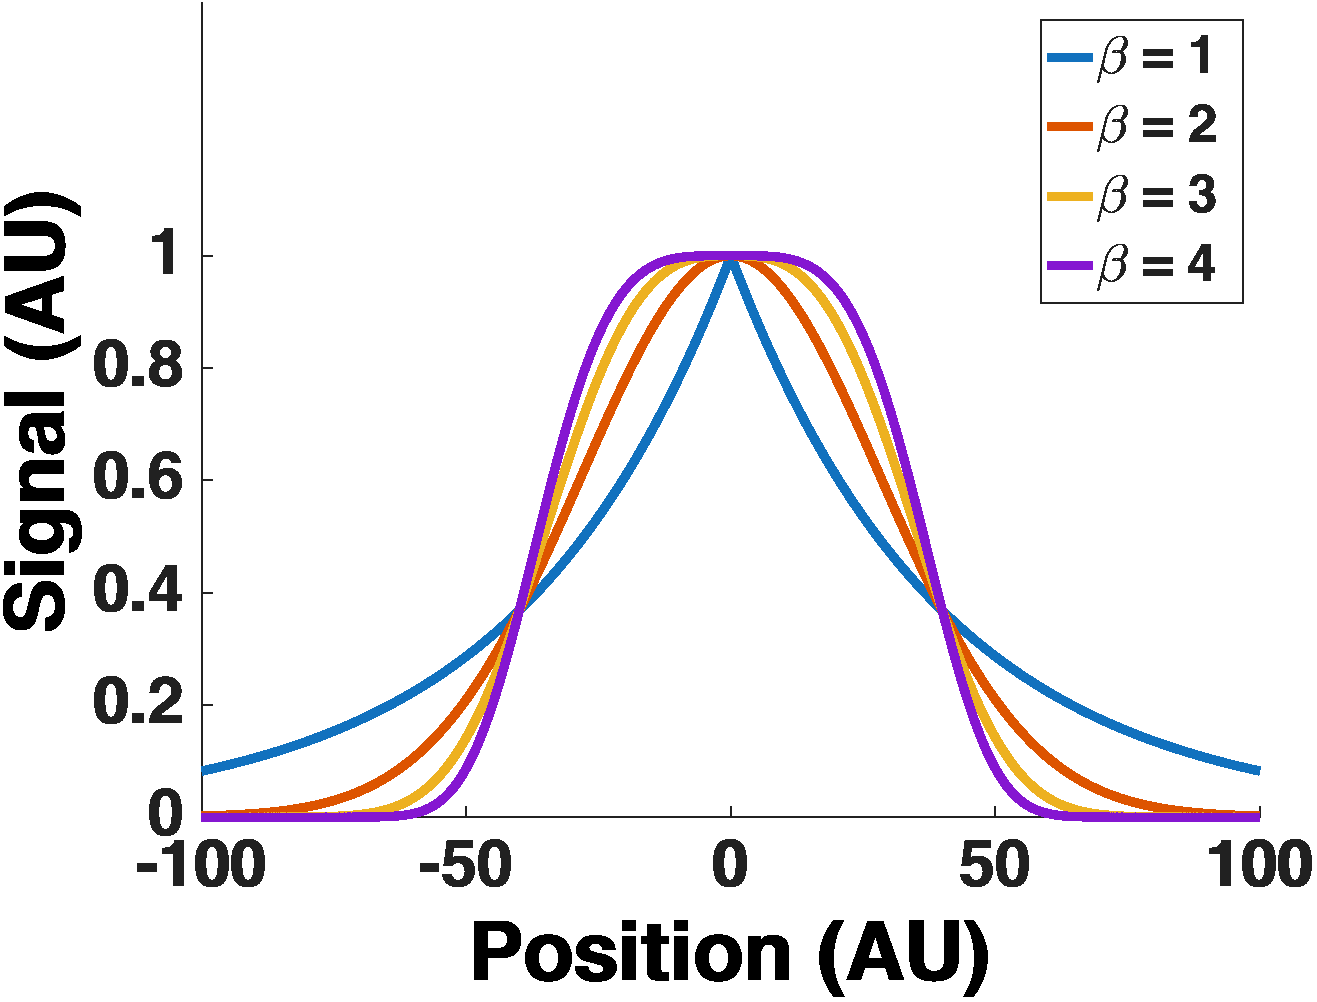
\includegraphics[height=3.8cm,keepaspectratio]{figures/gg_model_a.pdf}\end{subfigure}\hspace{0.02\linewidth}%
\begin{subfigure}[t]{0.38\linewidth}\centering\captionsetup{margin={6.25mm,0mm}}\caption{Model fits to MIP}\label{fig:gg_model_b}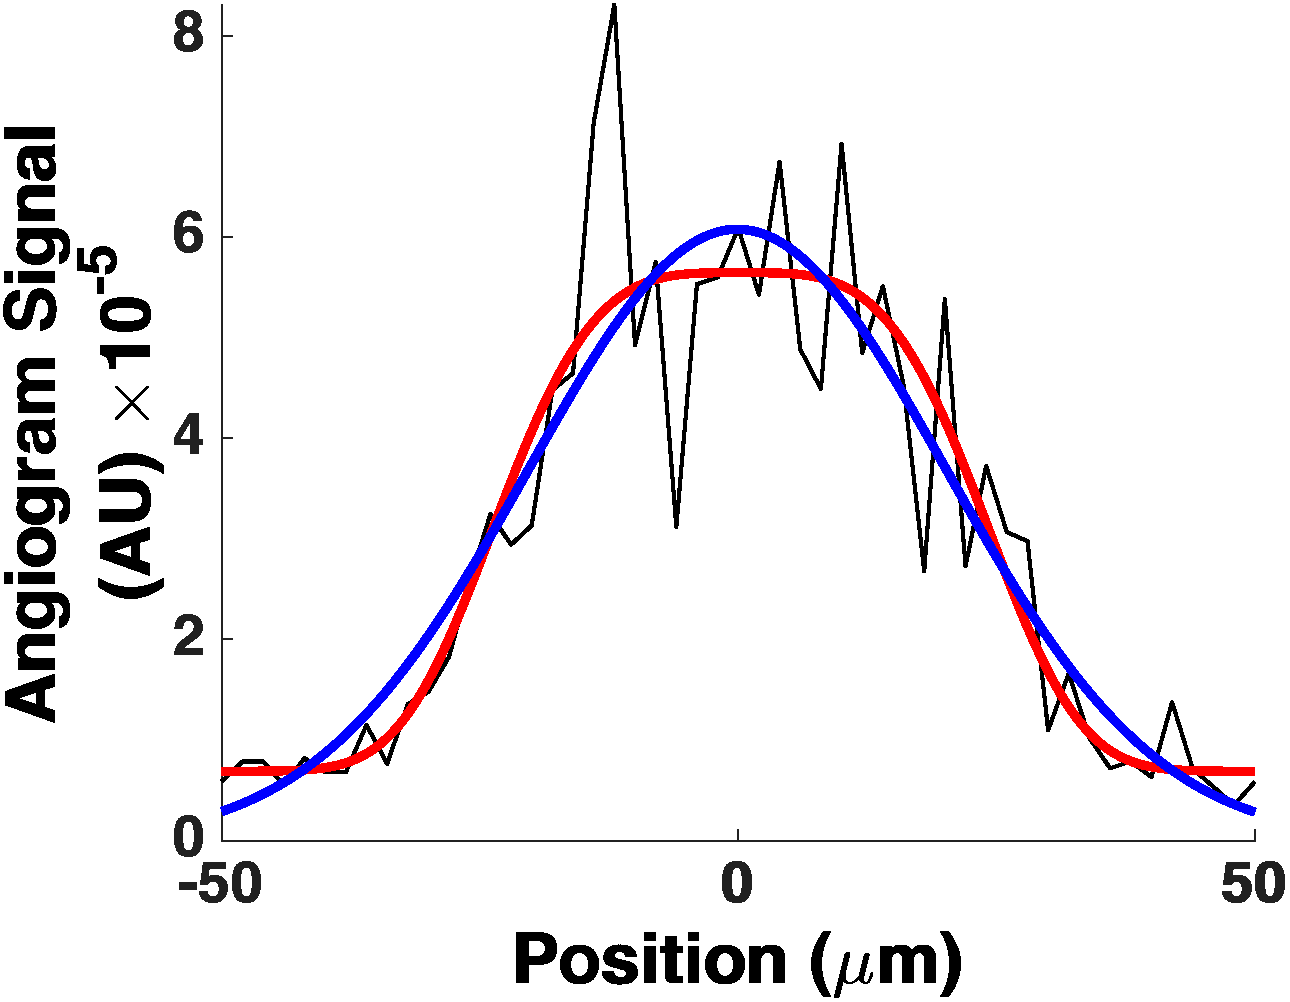
\includegraphics[height=3.8cm,keepaspectratio]{figures/gg_model_c.pdf}\end{subfigure}
\caption{(a) GG function for shape parameters $\beta = 1$, 2, 3, and 4.~(b) Example vessel intensity profile (black) taken from a MIP, with standard Gaussian (blue) and GG (red) fits. The MIP profile is flat-topped ($\beta = 9.9$), a shape the standard Gaussian cannot represent.}
\label{fig:gg_model}
\end{figure}

Two standard width metrics were calculated from the fitted models: the full width at half maximum (FWHM) and the $1/e^2$ width. For the standard Gaussian fit, the $1/e^2$ width was calculated as:
\begin{equation}
\label{eq:gauss_1e2}
w_{1/e^2,\,\mathrm{G}} = 4\sigma
\end{equation}
The FWHM for a Gaussian is related to the $1/e^2$ width by a fixed proportionality:
\begin{equation}
\label{eq:gauss_fwhm}
w_{fwhm,\,\mathrm{G}} = 2\sigma\sqrt{2\ln 2} = \frac{\sqrt{2\ln 2}}{2} \; w_{1/e^2,\,\mathrm{G}}
\end{equation}
and therefore only the $1/e^2$ width was calculated directly from the fit, with the FWHM obtainable via this known relationship.

For the GG fit, no such linear relationship exists between the FWHM and $1/e^2$ width, since both depend on the shape parameter $\beta$. Both metrics were therefore calculated independently as:
\begin{equation}
\label{eq:gg_fwhm}
w_{fwhm,\,\mathrm{GG}} = 2\alpha{\left(\ln 2\right)}^{1/\beta}
\end{equation}
\begin{equation}
\label{eq:gg_1e2}
w_{1/e^2,\,\mathrm{GG}} = 2\alpha \cdot 2^{1/\beta}
\end{equation}

\subsubsection{Binary mask based vessel diameter calculation}
\label{subsubsec:binary_mask}
For comparison with OCTA processing pipelines that rely on image binarisation, vessel diameters were also measured from binary masks generated by global thresholding. To determine the threshold level, the maximum angiogram intensity was measured after applying a 3D averaging filter with a kernel size of 50~$\times$~50~$\times$~10 voxels (lateral~$x$~$\times$~axial~$z$~$\times$~temporal~$t$) to the DyC-OCT angiogram volumes to reduce noise and minimize the effects of outliers. To produce a binarised black and white (BW) mask, the maximum angiogram intensity within these smoothed volumes were calculated, and five different threshold values were defined as fixed percentages of these maxima for MIP and MeIP. For MIP, the thresholds were defined as BW-1~=~40\%, BW-2~=~50\%, BW-3~=~60\%, BW-4~=~70\%, and BW-5~=~80\%. While for MeIP, the thresholds were defined as BW-1~=~07\%, BW-2~=~08\%, BW-3~=~09\%, BW-4~=~10\%, and BW-5~=~11\%.~These thresholds were selected empirically to cover the usable range of each projection. The upper and lower bounds were selected based on the point at which vessels began to be lost, and at which background noise and tissue signal were increasingly included, respectively. Each threshold was applied to the unsmoothed en face projection (MIP and MeIP) to generate a binary mask, and the vessel diameter was measured as the number of pixels above the threshold across the lateral vessel cross-section.

\subsubsection{Statistical analysis}
\label{subsubsec:stats}
To evaluate the accuracy and precision of all diameter measurement approaches, the calculated diameter values were plotted against the ground truth for each vessel across three conditions: pre-contrast, peak contrast, and post-contrast. A linear regression was fitted to each condition, yielding the slope ($m$) and coefficient of determination ($R^2$). A slope of $m = 1$ indicated perfect agreement with the ground truth, and $R^2$ quantified the goodness of fit of the linear model. Additionally, the coefficient of variation (CoV) was computed for each vessel across the time samples within each contrast condition and then averaged across vessels, to assess measurement precision (repeatability). For the model-based methods, six combinations were evaluated: two projection methods (MIP and MeIP) by three width metrics ($w_{1/e^2,\,\mathrm{G}}$, $\mathrm{FWHM}_{\mathrm{GG}}$, and $w_{1/e^2,\,\mathrm{GG}}$). For the binary mask based method, diameter was measured at five threshold levels (BW-1 through BW-5) for both MIP and MeIP. For the functional flicker stimulation experiment, a paired t-test was used to evaluate if stimulation induced changes were significant, and the Pearson correlation coefficient ($\rho$) between measured diameter values and angiogram intensity was computed for each method and vessel to assess whether the diameter measurements were affected by changes in angiogram intensity. Measurements with $p < 0.05$ were considered statistically significant (significance levels: $^{*}p < 0.05$, $^{**}p < 0.01$, $^{***}p < 0.001$). A paired t-test was used to evaluate whether vessel diameters differed significantly between the pre- and post-stimulation windows.